\section{Introduction}

A major trend in urban planning is the development of light rail transit networks to improve mobility and reduce road congestion. However, in cities where urban growth has historically been car-oriented, low residential and activity densities often make it challenging to achieve high transit ridership. To address this, park-and-ride (P\&R) facilities are commonly implemented near transit stations, enabling travelers to access the transit network by car for part of their journey.

Sioux Falls, South Dakota, is a rapidly growing city whose population has increased from 125,000 at the start of the century to over 200,000 today, spread across 210 km$^2$\footnote{\url{https://en.wikipedia.org/wiki/Sioux_Falls,_South_Dakota}}. For comparison, Geneva, Switzerland, has a similar population but a much denser public transport system, including multiple light rail and suburban train lines, and a dense bus network, despite covering only 16 km$^2$\footnote{\url{https://fr.wikipedia.org/wiki/Gen\%C3\%A8ve}}. In contrast, Sioux Falls' public transportation consists of just 9 bus lines operating 6 days a week, supplemented by on-demand services\footnote{\url{https://siouxareametro.info/bus}}. The city’s road network is also notable as the basis for a widely used benchmark in traffic engineering, due to its manageable size and typical grid structure.

\begin{figure}
    \centering
    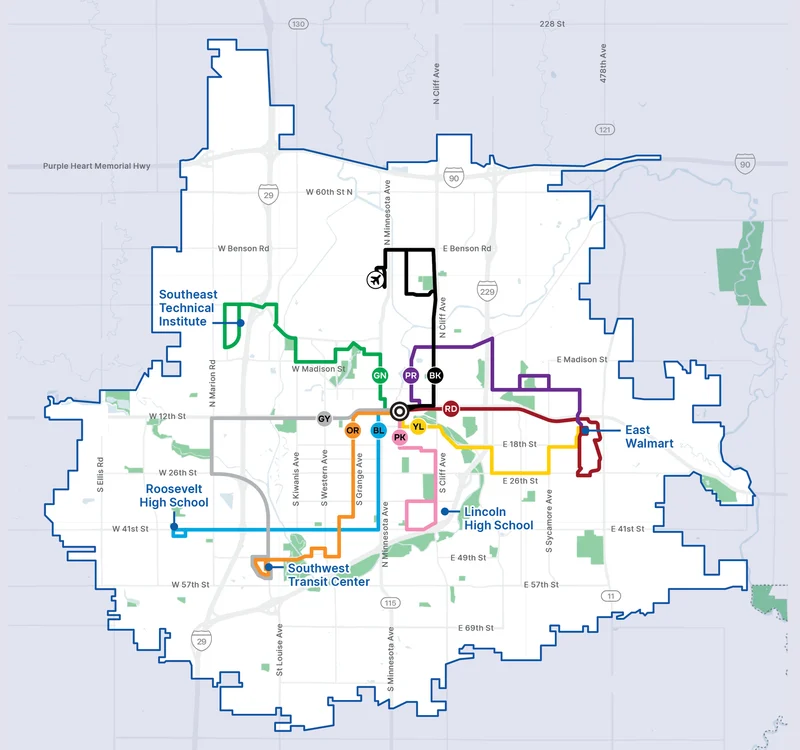
\includegraphics[keepaspectratio,width=0.45\textwidth]{Figures/siouxfalls_bus_network.png}
    \caption{Sioux Falls' current bus network.}
    \label{fig:sioux_falls_bus_network}
\end{figure}

This study explores a hypothetical scenario in which Sioux Falls introduces a light rail network to enhance public transportation. Specifically, we analyze the potential reduction in road traffic resulting from converting parts of the existing bus network to light rail and from adding park-and-ride facilities at stations. We model traffic assignment at \textit{User Equilibrium} (UE) on the benchmark network, first simulating the new light rail lines as additional links available only to users whose origin and destination are both on the line. We then relax this constraint to allow access if either the origin or destination is on the line, representing the effect of P\&R facilities.

Future research could extend this analysis by considering parking and ticket costs, the inconvenience and time associated with transfers, and waiting times as additional generalized costs. Other possible extensions include limiting P\&R facilities to selected stations, imposing parking capacity constraints, refining cost calculations (e.g., including fuel costs), and conducting sensitivity analyses on these parameters.